\section{Analyse des performances vis-à-vis des mouvements respiratoires}
\begin{obj}
Quantifier le niveau de performance de la loi de commande déterminée en considérant la consigne correspondant aux mouvements physiologiques. Une amélioration de la loi de commande est ensuite envisagée sous la forme d'une anticipation sur la consigne pour améliorer les performances.
\end{obj}

Cette partie porte sur l'analyse et l'amélioration des performances vis-à-vis des signaux respiratoires. Pour ce type de signaux, la consigne de position angulaire est modélisée par le signal $q_{j}^{*}(t)=B \sin (\omega t)$ où l'amplitude $B$ (comprise entre 0,04 et $\SI{0,09}{rad}$ ) et la pulsation $\omega$ (comprise entre les deux valeurs $\omega_{1}$ et $\omega_{2}$ ) sont calculées à partir des deux termes sinusoïdaux retenus dans la partie I.A. On considère le schéma de la figure \ref{fig_11}, on suppose que la structure de correction permet d'assurer la pulsation propre $\omega_{0}$ souhaitée en boucle fermée et que les perturbations extérieures sont nulles $\left(C_{\text {ext }}=0\right)$.\\

%Q 30. 
\question{La fonction de transfert de la consigne $Q_{j}^{*}(p)$ vers l'écart $\varepsilon(p)$, obtenue à partir du schéma bloc de la figure \ref{fig_11}, peut être approchée dans la bande de pulsations $\omega \ll \omega_{0}$, caractéristique des signaux de consigne, par la relation $\frac{\varepsilon(p)}{Q_{j}^{*}(p)} \approx 0,066 p$. En utilisant cette approximation, calculer l'amplitude de l'écart en régime permanent vis-à-vis des deux termes de consigne sinusoïdaux retenus pour modéliser les mouvements respiratoires. Conclure sur cette performance comparativement aux exigences de précision du cahier des charges exprimées dans la figure \ref{fig_12}.}
\ifprof
\begin{corrige}
Pour un signal périodique en entrée d'amplitude $B$, l'écart sera un signal périodique d'amplitude $0,066\cdot B\cdot \omega_i$, avec $i=\left\{1,2\right\}$ et $\omega_i=2\pi f_i$ ($f_1=0,24Hz$ et $f_2=0,48Hz$).
On note $\varepsilon_0$ l'amplitude de l'écart en régime permanent.

\begin{center}
\begin{tabular}{|c|c|c|}
\hline 
$f_i$ & $f_1$ & $f_2$ \\ 
\hline 
$\varepsilon_0$  & $0,066\cdot 2\pi f_1$ & $0,066\cdot 2\pi f_2$ \\ 
\hline 
Application numérique sur $\dfrac{\varepsilon_0}{B}$ & \SI{9,95e-2}{} & \SI{19,91e-2}{} \\ 
\hline 
\end{tabular} 
\end{center}
 
Ces valeurs ne sont pas conformes au cahier des charges car l'exigence 5.2.2 impose : $\dfrac{\varepsilon_j}{B_j}<10^{-2}$.
\end{corrige}
\else
\fi


Afin d'améliorer ce niveau de performance, on complète la loi de commande en ajoutant un terme d'anticipation $c_{a}(t)$ selon la structure de commande représentée d'un point de vue symbolique par le schéma de la figure \ref{fig_15} (pour cette partie, on ne tiendra pas compte des perturbations, seule la structure représentée sur ce schéma bloc sera considérée). La conception de ce terme d'anticipation est l'objectif de la suite de l'étude.

\begin{figure}[!h]
\centering
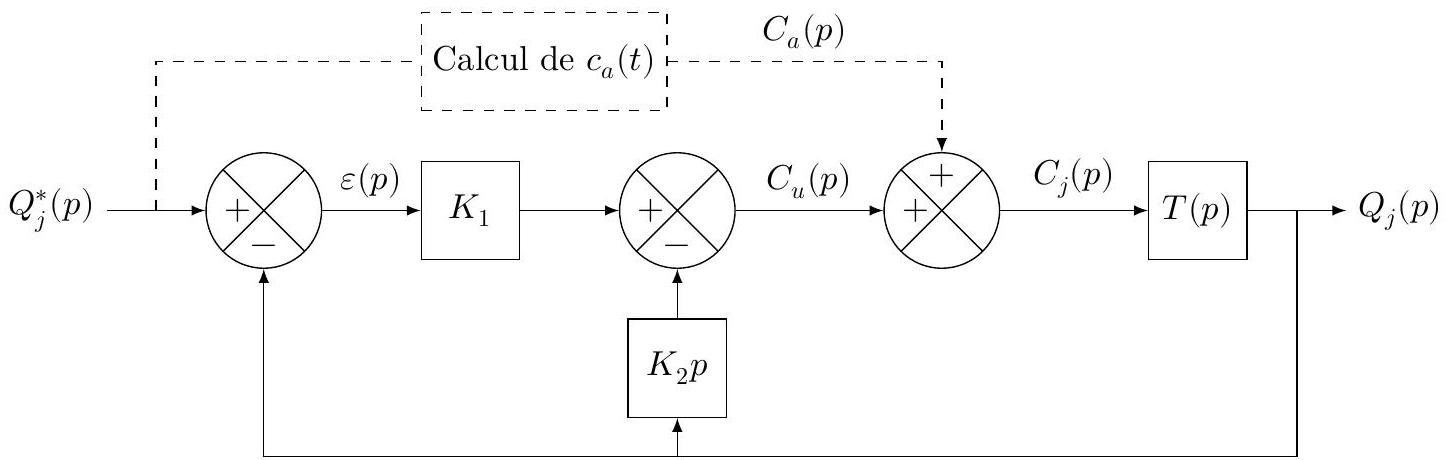
\includegraphics[width=.9\textwidth]{2024_08_29_b4f920ed3822451bf72bg-13}
\caption{\label{fig_15} Structure de commande avec anticipation sur la consigne}
\end{figure}

%Q 31. 
\question{En utilisant les différents éléments de la structure représentée, en particulier la fonction de transfert $T(p)=\frac{Q_{j}(p)}{C_{j}(p)}$, et en supposant que la consigne est idéalement suivie sans erreur, c'est à dire $q_{j}(t) \equiv q_{j}^{*}(t)$, donner en fonction de $q_{j}^{*}(t)$ et de ses dérivées l'expression temporelle du couple idéal $c_{j}(t)$ et du couple $c_{u}(t)$ issu du correcteur. En déduire alors l'expression du terme d'anticipation $c_{a}(t)$ qu'il est nécessaire d'ajouter pour obtenir le comportement souhaité.}
\ifprof
\begin{corrige}
\begin{itemize}
\item \textbf{Expression temporelle du couple idéal $c_j(t)$ : }
d'après le schéma bloc dans le domaine de Laplace : $C_j(p)=\dfrac{Q_j(p)}{T(p)}=\indice{J}{eq}p^2Q_j(p)$, en repassant dans le domaine temporel : 
$
c_j(t)=\indice{J}{eq}\dfrac{\dd ^2q_j(t)}{\dd t^2}=\indice{J}{eq}\dfrac{\dd ^2q^*_j(t)}{\dd t^2}
$;
\item \textbf{Expression temporelle du couple idéal $c_u(t)$ : }
d'après le schéma bloc dans le domaine de Laplace : $C_u(p)=K_1\cdot (Q^*_j(p)-Q_j(p))-K_2\cdot p\cdot Q_j(p)=-K_2\cdot p\cdot Q^*_j(p)$, en repassant dans le domaine temporel : 
$
c_u(t)=-K_{2}\dfrac{\dd q^*_j(t)}{\dd t}$;
\item au niveau du comparateur on lit : $c_a(t)=c_j(t)-c_u(t)$, ainsi $c_a(t)=\indice{J}{eq}\dfrac{\dd ^2q^*_j(t)}{\dd t^2}+K_{2}\dfrac{\dd q^*_j(t)}{\dd t}$.
\end{itemize}
\end{corrige}
\else
\fi


La structure de commande avec anticipation sur la consigne peut être réalisée selon le schéma bloc de la figure \ref{fig_16}.

\begin{figure}[!h]
\centering
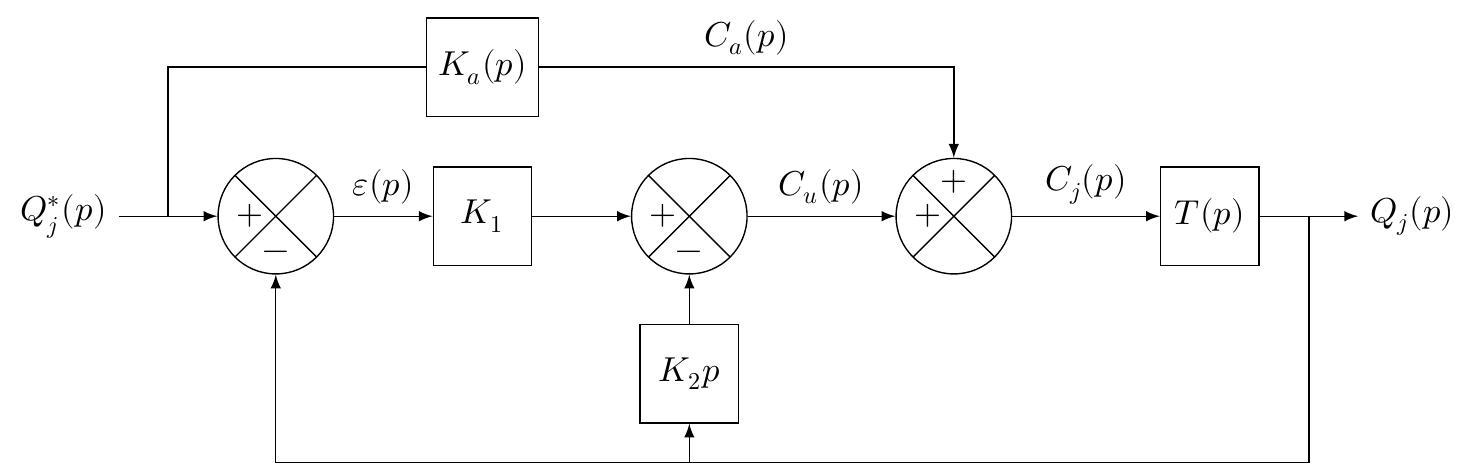
\includegraphics[width=.9\textwidth]{2024_08_29_b4f920ed3822451bf72bg-13(1)}
\caption{\label{fig_16} Structure de commande avec anticipation sur consigne}
\end{figure}


%Q 32. 
\question{Au regard de cette représentation (figure \ref{fig_16}):}
\textit{\begin{itemize}
  \item déterminer la fonction de transfert du correcteur par anticipation $K_{a}(p)$;
  \item déterminer la fonction de transfert en boucle fermée $F(p)=\frac{Q_{j}(p)}{Q_{j}^{*}(p}$. Justifier alors que l'erreur est nulle vis-à-vis de la consigne et en particulier vis-à-vis de signaux de consigne sinusoïdaux.\\
\end{itemize}}
\ifprof
\begin{corrige}
\begin{itemize}
\item \textbf{Détermination de $K_a(p)$ :} on déduit de la question précédente (en supposant les conditions initiales nulles) : $K_a(p)=\dfrac{C_a(p)}{Q^*_j(p)}=\indice{J}{eq}\cdot p^2+K_2\cdot p$.
\item \textbf{Détermination de $F(p)$ :}
\end{itemize}

On a $Q_j(p) = C_j(p) T(p)= \left( Q_j^{\star}(p) K_a(p) + C_u(p) \right) T(p)$
$= \left( Q_j^{\star}(p) K_a(p) + C_u(p) \right) T(p)$

$= \left( Q_j^{\star}(p) K_a(p) + \left( \varepsilon(p) K_1 - K_2 p Q_j(p) \right)\right) T(p)$

$= \left( Q_j^{\star}(p) K_a(p) + \left( \left(Q_j^{\star}(p) - Q_j(p) \right) K_1 - K_2 p Q_j(p) \right)\right) T(p)$

%$Q_j(p) = \left( Q_j^{\star}(p) K_a(p) + \left( \left(Q_j^{\star}(p) - Q_j(p) \right) K_1 - K_2 p Q_j(p) \right)\right) T(p)$

$\Leftrightarrow Q_j(p) = 
\left(
    Q_j^{\star}(p) K_a(p) + 
    \left( 
        \left(Q_j^{\star}(p) - Q_j(p) \right) K_1 - K_2 p Q_j(p) 
    \right)
\right) T(p)$

$\Leftrightarrow Q_j(p) = 
    T(p)Q_j^{\star}(p) K_a(p) + 
    T(p)\left( 
        \left(Q_j^{\star}(p) - Q_j(p) \right) K_1 - K_2 p Q_j(p) 
    \right) $

$\Leftrightarrow Q_j(p) = 
    T(p)Q_j^{\star}(p) K_a(p) + 
        T(p)K_1 Q_j^{\star}(p) -T(p)K_1  Q_j(p)   - T(p)K_2 p Q_j(p) 
     $

$\Leftrightarrow Q_j(p)\left(1     +T(p)K_1     + T(p)K_2 p\right)= 
      Q_j^{\star}(p)T(p) \left(  K_a(p)     +K_1 \right)     $

On a donc $F(p)=\dfrac{Q_j(p)}{Q_j^{\star}(p)}=\dfrac{\left(K_a(p) +K_1\right)T(p)}{1+T(p)K_1 + T(p)K_2 p}$.
En factorisant par $T(p)$ au numérateur et au dénominateur puis en remplaçant $T(p)$ par $\dfrac{1}{\indice{J}{eq}p^2}$ et $K_a(p)=\indice{J}{eq}\cdot p^2+K_2\cdot p$, on obtient $
F(p)=\dfrac{\indice{J}{eq}p^2+K_1+K_2\cdot p}{\indice{J}{eq}p^2+K_1+K_2\cdot p}=1
$.

Ainsi quelle que soit la forme de l'entrée, $Q^*_j(p)=Q_j(p)$ et donc l'erreur est nulle en particulier vis-à-vis de signaux de consigne sinusoïdaux.
\end{corrige}
\else
\fi

Une fonction telle que $K_{a}(p)$ est difficile à réaliser en pratique, voire impossible. La réalisation de la loi de commande est numérique et on implante cette loi de commande selon la structure de la figure \ref{fig_17} en séparant le mouvement périodique dû à la respiration $\delta q_{j}^{*}(t)=B_{1} \sin \left(\omega_{1} t+\theta_{1}\right)+B_{2} \sin \left(\omega_{2} t+\theta_{2}\right)$ de la partie due à la consigne correspondant au point de fonctionnement $Q_{j 0}^{*}(p)$.


\begin{figure}[!h]
\centering
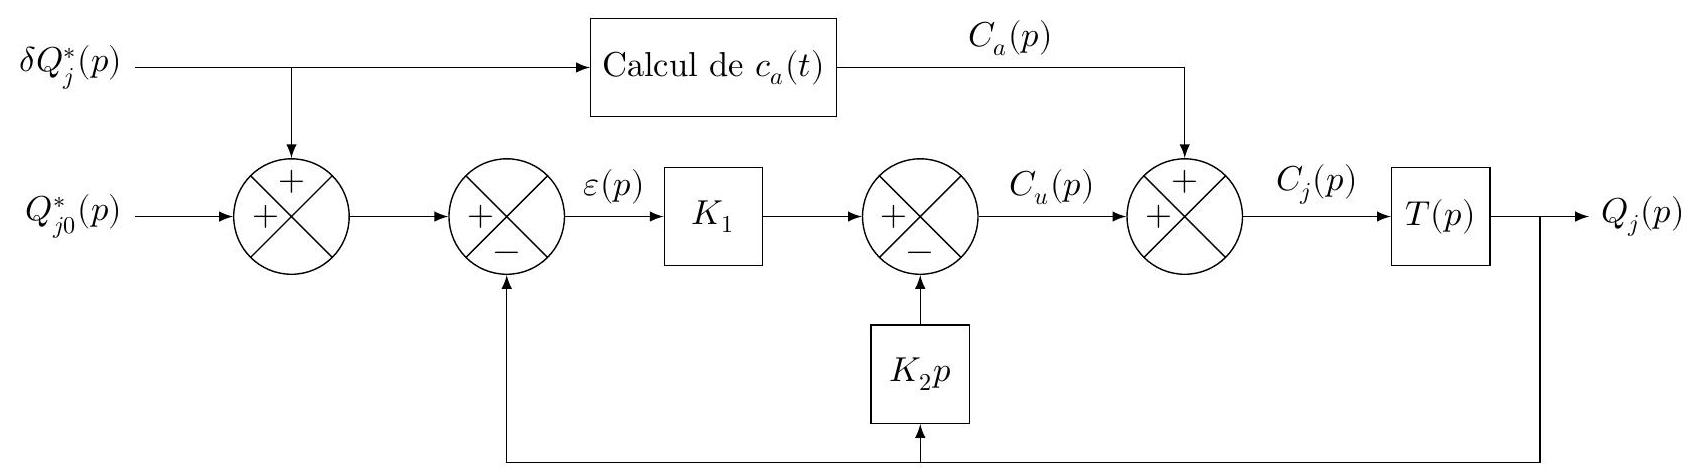
\includegraphics[width=.8\textwidth]{2024_08_29_b4f920ed3822451bf72bg-14}
\caption{\label{fig_17} Schéma d'implantation de la structure de commande avec anticipation sur la consigne}
\end{figure}

%Q 33. 
\question{Donner alors l'équation permettant de calculer le signal d'anticipation $c_{a}(t)$ pour le cas du signal $\delta q_{j}^{*}(t)$ sinusoïdal retenu pour modéliser les mouvements physiologiques.}
\ifprof
\begin{corrige}
En reprenant le résultat de la question 31 qui permet d'exprimer $c_a(t)$ dans le domaine temporel, on obtient, $
c_a(t)=\indice{J}{eq}\dfrac{\dd ^2\delta q^*_j(t)}{\dd t^2}+K_{2}\dfrac{\dd \delta q^*_j(t)}{\dd t}$
$=-\indice{J}{eq}\omega_1^2B_1\sin\left(\omega_1t+\theta_1\right)+K_2\omega_2B_2\cos\left(\omega_2t+\theta_2\right)
$.
\end{corrige}
\else
\fi


\paragraph*{Question de synthèse}

En adoptant cette stratégie de commande :
\begin{itemize}
  \item la figure \ref{fig_18} montre le déplacement de la position angulaire de l'axe 3 en réponse à une variation en échelon d'amplitude $\SI{0,3}{rad}$ de la consigne ;
  \item la figure \ref{fig_19} montre les évolutions de la consigne sinusoïdale destinée à suivre les mouvements physiologiques, de la sortie et du signal d'écart associé.
\end{itemize}

\begin{figure}[!h]
\centering
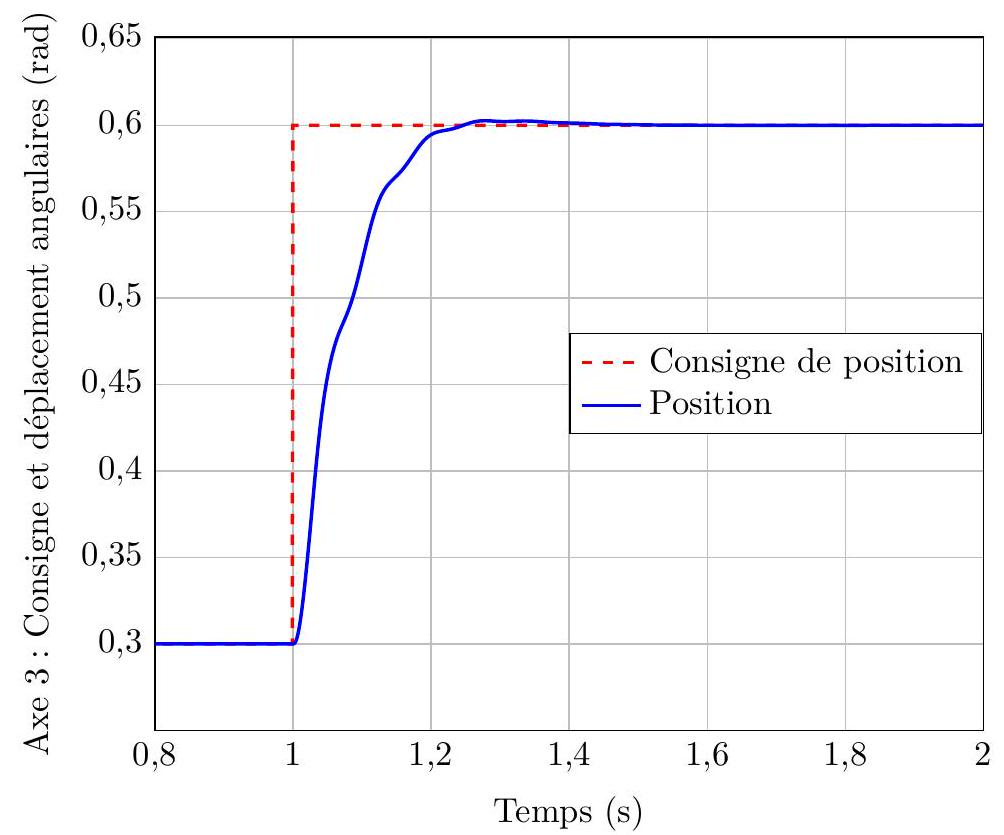
\includegraphics[max width=.7\textwidth]{2024_08_29_b4f920ed3822451bf72bg-14(1)}

\caption{\label{fig_18} Axe 3 : réponse à une variation en échelon d'amplitude $0,3 \mathrm{rad}$ de la consigne de position articulaire}
\end{figure}

%Q 34. 
\question{Analyser les réponses obtenues et conclure (en argumentant la réponse) sur la pertinence de ce système au regard de la problématique de compensation des mouvements physiologiques pour les robots de téléopération en chirurgie mini-invasive.}
\ifprof
\begin{corrige}
\begin{itemize}
\item Sur la figure 18, on peut juger des performances liées aux exigences 1.2 ("Asservissement au point de fonctionnement") :
\begin{itemize}
\item \textbf{Précision :} La précision obtenue est optimale. La position angulaire obtenue est confondu à la consigne en régime permanent ce qui se traduira par un écart en régime permanent inférieur à $10\mu m$.
\item \textbf{Rapidité : } le temps de réponse à $5\%$ est la durée entre l'instant de l'échelon et l'instant au delà duquel la position est comprise entre $\pm 5\%$ de la valeur finale et qui correspond ici à la durée au delà de laquelle la position est comprise entre $0,57\mu m$ et $0,63\mu m$. Sur la figure 18, on relève approximativement $\SI{0,15}{s}<\SI{0,2}{s}$ comme l'exige l'exigence 1.2.2.  
\end{itemize}
\item Sur la figure 19, on peut juger des performances liées aux exigences 1.3 ("Suivi des mouvements physiologiques"). 
\begin{itemize}
\item le signal de consigne possède une fréquence d'environ $\SI{0,5}{Hz}$ et une amplitude de consigne $\SI{0,34}{rad}$. 
\item l'erreur relatif est égale en amplitude à environ $\dfrac{75\times 10^{-6}}{0,34}\approx 2,2\times 10^{-4}<10^{-2}$ ce qui est bien conforme au cahier des charges.
\end{itemize}
\end{itemize}
\end{corrige}
\else
\fi
\begin{figure}[!h]
\centering
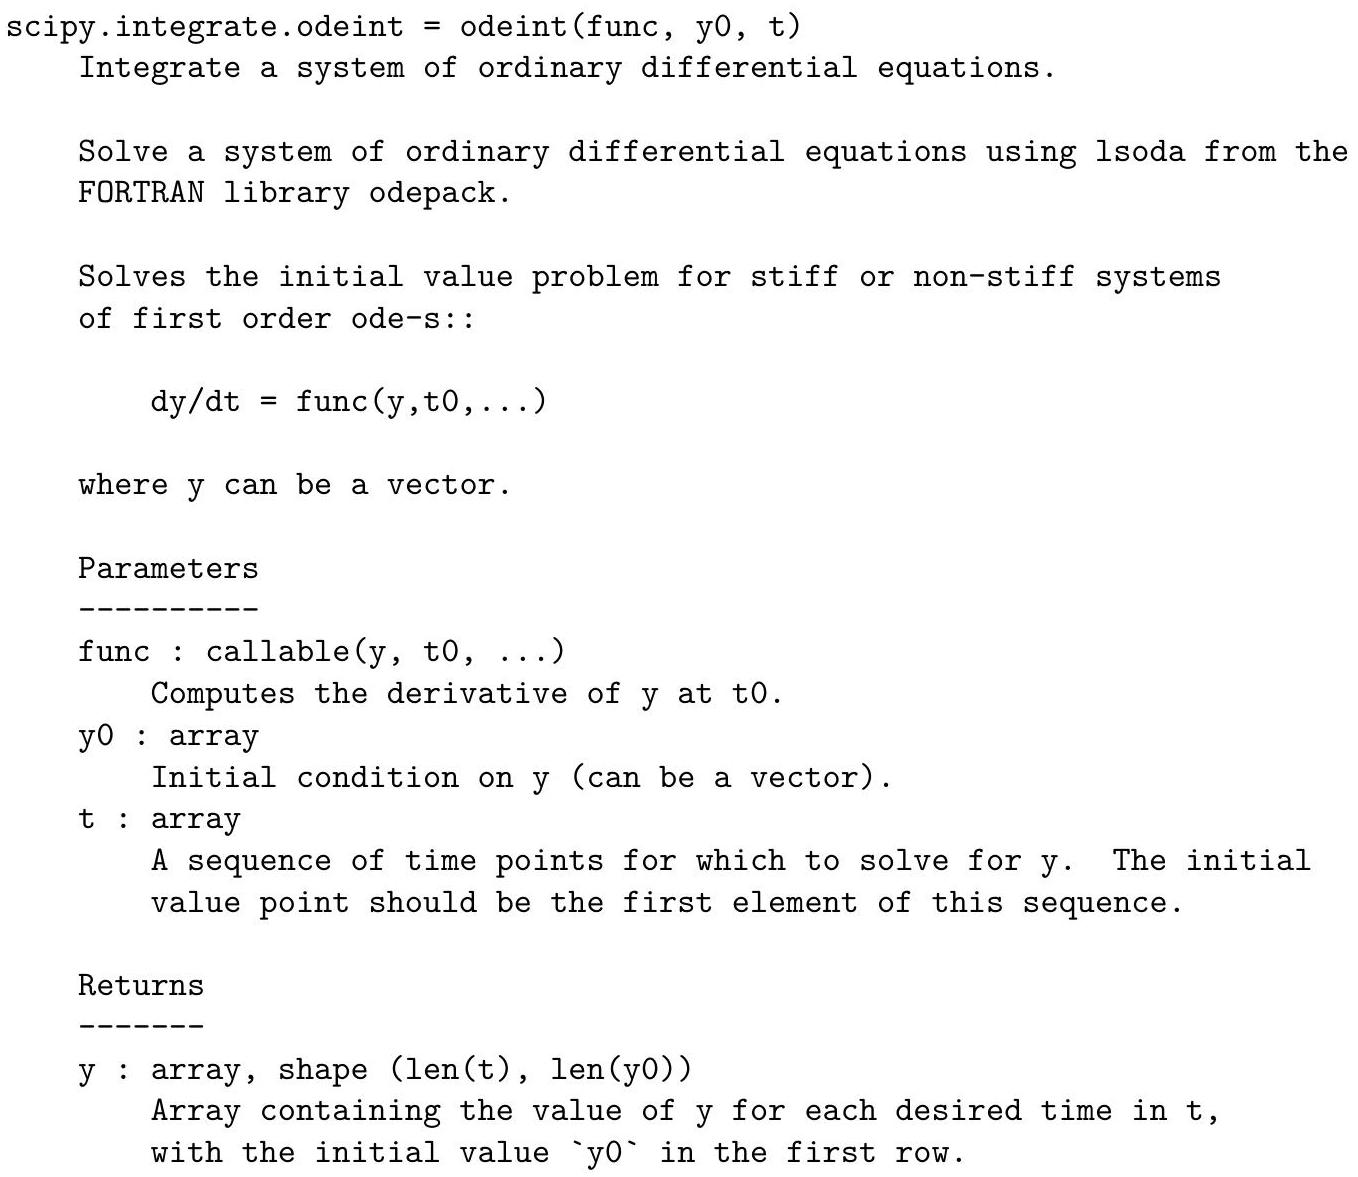
\includegraphics[width=\textwidth]{fig_19}

\caption{\label{fig_19} Axe 3 : réponse à une consigne sinusoïdale de la position angulaire de l’articulation}
\end{figure}